%==============================================================================
%  Note on the pre-ringing fix in SuperMoTo
%
%  Where the ringing around the peak of a sweep-deconvolved impulse response
%  actually comes from, which of the published remedies apply to this software
%  and which do not, the measurements that decided between them, and the two
%  places where the implementation departs from the plan it started with.
%
%  Build:  pdflatex note_on_pre-ringing_fix.tex   (twice, for references)
%
%  (c) 2023-2026 Olivier Doare - LGPL-3.0-or-later
%==============================================================================
\documentclass[11pt,a4paper]{article}

\usepackage[utf8]{inputenc}
\usepackage[T1]{fontenc}
\usepackage{lmodern}
\usepackage[margin=2.5cm]{geometry}
\usepackage{amsmath}
\usepackage{amssymb}
\usepackage{booktabs}
\usepackage{tabularx}
\usepackage{enumitem}
\usepackage{xcolor}
\usepackage{tikz}
\usetikzlibrary{positioning,arrows.meta,calc,fit,backgrounds}
\usepackage{pgfplots}
\pgfplotsset{compat=1.17}
\usepackage{siunitx}
\DeclareSIUnit{\dB}{dB}
\usepackage{fancyhdr}

\definecolor{smtblue}{HTML}{2E6DB4}
\definecolor{smtgold}{HTML}{C9A227}
\definecolor{smtgreen}{HTML}{3FA34D}
\definecolor{smtred}{HTML}{B4472E}
\definecolor{smtpanel}{HTML}{2B2F36}

\usepackage[colorlinks=true,linkcolor=smtblue,urlcolor=smtblue]{hyperref}

\pagestyle{fancy}
\fancyhf{}
\fancyhead[L]{\small Note on the pre-ringing fix}
\fancyhead[R]{\small SuperMoTo}
\fancyfoot[C]{\thepage}
\renewcommand{\headrulewidth}{0.4pt}

% Code references: \srcref{file}{line}. The \discretionary lets TeX break
% between the file name and the line number rather than overrunning the margin.
\newcommand{\srcref}[2]{\texttt{\small #1}\discretionary{}{}{}\texttt{\small :#2}}
\newcommand{\code}[1]{\texttt{\small #1}}

% Typewriter identifiers do not hyphenate; give the line breaker room instead of
% letting them overrun the margin.
\setlength{\emergencystretch}{3em}

% A boxed remark
\newenvironment{remark}[1]
  {\par\medskip\noindent\begin{tabular}{@{}p{0.03\textwidth}p{0.93\textwidth}@{}}
   \textcolor{smtblue}{\rule{2pt}{\baselineskip}} & \textbf{#1}\\[2pt] & \ignorespaces}
  {\end{tabular}\par\medskip}

\title{\bfseries Note on the pre-ringing fix in SuperMoTo\\
       \large Which published remedy applies, which does not, and what the
       measurements decided}
\author{}
\date{September 2026}

\begin{document}
\maketitle
\thispagestyle{fancy}

\begin{abstract}
\noindent
The impulse responses SuperMoTo recovers by deconvolving a logarithmic sweep
carry a symmetric ringing around their peak. The literature on the exponential
sine sweep attributes such ringing mainly to the fade-out applied to the test
signal, and offers three remedies: remove the fade-out, cut the sweep at its
last zero crossing, and repair what is left with a regularised inverse
``packing'' filter built from a loopback reference.

Applied to this software, the first two of those remedies are worth almost
nothing and the third is worth little. The ringing here is not a fade artefact
at all: it is the sinc of the stimulus band edge at \SI{20}{\kilo\hertz}, and it
is made worse, not better, by every increase in sample rate. This note derives
why, gives the loopback measurements that separate the three candidate
mechanisms, and shows that one change accounts for essentially all of the
available improvement: running the sweep to Nyquist over a whole number of
octaves, which is worth about \SI{43}{\dB} at \SI{48}{\kilo\hertz}.

Two decisions taken during implementation contradict the plan the work started
from, and both are recorded here with the measurements that forced them.
Truncating at the last zero crossing was dropped, because a sweep that ends at
Nyquist has no zero crossing to cut to. The fade-out was therefore shortened
rather than removed, because the alternative is a near-full-scale step into the
tweeter. Sections~\ref{sec:impl} and~\ref{sec:notdone} describe code that is now
in the software.
\end{abstract}

\tableofcontents
\bigskip

%==============================================================================
\section{Purpose and scope}

This note covers the stimulus that SuperMoTo emits and the deconvolution that
turns a recording of it back into an impulse response. It is concerned with one
defect only: the ringing that surrounds the peak of that impulse response and
that is visible on the impulse view of the Analysis and Group analysis panes.

It does \emph{not} cover the design of the correction filters. That design has
its own inversion problem, and Section~\ref{sec:notdone} explains why the
regularisation literature that looks most relevant to it turns out not to
improve it.

Everything measured here uses the Farina/Novak sweep path, that is
\code{AnalysisEngine::}\allowbreak\code{TfMethod::sweep}. The Welch path
estimates the transfer function from cross- and auto-spectra of Hann-windowed
segments, and never deconvolves anything, so none of what follows applies
to it.

%==============================================================================
\section{Relation to existing work}

\subsection{What the literature covers}

Farina's 2007 paper \cite{Farina2007} is the direct source for the problem. Its
Section~3.1 lists pre-ringing before the arrival of the direct sound as the
first of five defects of the exponential sine sweep method, and proposes, in
order: removing the fade-out, continuing the sweep up to the Nyquist frequency
and cutting it manually at the latest zero crossing before its termination, and
finally, for the low-frequency pre-ringing that analogue equipment contributes,
a ``packing'' filter computed by the Kirkeby method from a reference
measurement. The underlying regularised inversion is
Kirkeby, Rubak and Farina \cite{Kirkeby1998}, whose contribution is the
frequency-dependent regularisation parameter that keeps the inverse filter's
time response short.

Vetter and di Rosario \cite{Vetter2011} attack the same problem from the
stimulus side. Their observation is the useful one for us: a fade-\emph{out} is
represented in the deconvolved chirp by filter coefficients of substantial value
around the central pulse, whereas a fade-\emph{in} is not. Rather than cutting
by hand, they define a phase-controlled chirp spanning an integer number of
octaves with Nyquist as the stop frequency, which ends in sine phase by
construction, and they add an optional fade-in one octave long.

Novak, Lotton and Simon \cite{Novak2015} supply the synchronized sweep that this
software already uses, and the analytic inverse this note works with. Farina's
earlier paper \cite{Farina2000} introduces the swept-sine measurement of impulse
response and distortion together. Mosleh, Langlois and Green \cite{Mosleh2014}
treat deconvolution ringing in image deblurring; it is included for completeness
and discussed in Section~\ref{sec:notdone}.

\subsection{What this note adds}

Three things.

First, an attribution. The published discussion assumes the fade-out is the
dominant cause. With SuperMoTo's parameters it is not, and
Section~\ref{sec:mechanisms} separates the three candidate mechanisms and
measures each one.

Second, a negative result with a proof. Farina's second remedy, cutting at the
last zero crossing, becomes vacuous exactly when his first recommendation,
sweeping to Nyquist, is followed. Section~\ref{sec:nyquist-end} shows why the
two are incompatible and what to do instead.

Third, the observation that the analytic inverse in
\code{fxme::SynchronizedSweep::deconvolve} is applied unregularised over the
whole spectrum, together with the group-delay identity that says where
out-of-band content ends up, and a measurement of what that costs.

%==============================================================================
\section{The stimulus and its inverse}
\label{sec:stimulus}

\subsection{The synchronized sweep}

The emitted stimulus is
%
\begin{equation}
  x(t) \;=\; \sin\!\Bigl( 2\pi f_1 L \bigl( e^{t/L} - 1 \bigr) \Bigr),
  \qquad 0 \le t \le T,
  \label{eq:sweep}
\end{equation}
%
with the sweep rate $L$ quantised so that
%
\begin{equation}
  k \;\equiv\; f_1 L \;\in\; \mathbb{Z},
  \label{eq:novak}
\end{equation}
%
which is Novak's synchronization condition \cite{Novak2015}. The instantaneous
frequency is $f(t) = f_1 e^{t/L}$, so the sweep reaches frequency $f$ at
%
\begin{equation}
  t(f) \;=\; L \ln (f/f_1),
  \label{eq:arrival}
\end{equation}
%
and the total duration is $T = L \ln (f_2/f_1)$. This is generated sample by
sample in \code{MeasurementEngine::nextStimulusSample}.

\subsection{The analytic inverse and its group delay}

The recording is deconvolved not by a time-reversed copy of the stimulus but by
the analytic spectral inverse of \eqref{eq:sweep}, the stationary-phase
approximation of the sweep spectrum:
%
\begin{equation}
  \tilde X(f) \;=\; 2\sqrt{f/L}\;
    \exp\Bigl( -j\,2\pi f L \bigl( 1 - \ln (f/f_1) \bigr) + j\tfrac{\pi}{4} \Bigr).
  \label{eq:inverse}
\end{equation}
%
Write $\varphi(f)$ for that phase. Since
$\frac{d}{df}\bigl[ f (1 - \ln (f/f_1)) \bigr] = -\ln(f/f_1)$, we have
$d\varphi/df = 2\pi L \ln (f/f_1)$, and the group delay of the inverse filter is
%
\begin{equation}
  \tau(f) \;=\; -\frac{1}{2\pi}\,\frac{d\varphi}{df}
           \;=\; -\,L \ln (f/f_1) \;=\; -\,t(f).
  \label{eq:groupdelay}
\end{equation}
%
The inverse undoes exactly the dispersion that \eqref{eq:arrival} introduced.
Content that the sweep placed at frequency $f$ at time $t(f)$ is returned to
time zero, which is what makes the whole method work.

\begin{remark}{The identity holds whether or not the sweep put the content there}
Equation~\eqref{eq:groupdelay} is a property of the filter, not of the
recording. It is applied to \emph{everything} in the recording, including
content at frequencies the sweep never visited. That is the seed of
Section~\ref{sec:outofband}.
\end{remark}

Two properties of \eqref{eq:inverse} matter later. Its magnitude grows as
$\sqrt{f}$, without bound and without regard to the sweep's band. And in
\code{fxme::SynchronizedSweep::deconvolve} it is evaluated for every bin from
$k=1$ to $N/2$, that is from $f_s/N$ up to Nyquist, with no regularisation and
no band limit. Only the DC bin is zeroed.

%==============================================================================
\section{Three candidate mechanisms}
\label{sec:mechanisms}

Before the change, the stimulus ran from \SI{10}{\hertz} to
\SI{20}{\kilo\hertz} with a \SI{20}{\milli\second} linear fade at each end,
irrespective of sample rate. Three mechanisms could plausibly produce ringing
around the peak.

\subsection{The fade-out}

This is the one the literature emphasises. Its effect is easy to bound. The
instantaneous frequency at the end of the sweep advances at
$df/dt = f/L$, so a fade of duration $\Delta t$ tapers a band of width
$\Delta f \approx f_2 \Delta t / L$. For a \SI{10}{\second} sweep from
\SI{10}{\hertz} to \SI{20}{\kilo\hertz} at \SI{48}{\kilo\hertz}, quantisation
\eqref{eq:novak} gives $L = \SI{1.30}{\second}$, so the
\SI{20}{\milli\second} fade-out tapers
%
\begin{equation}
  \Delta f \;\approx\; \frac{20000 \times 0.02}{1.30} \;\approx\; \SI{308}{\hertz},
\end{equation}
%
that is from \SI{19695}{\hertz} to \SI{20}{\kilo\hertz}: a span of
\num{0.022} octave at the very top of an eleven-octave stimulus. The fade-in,
by the same argument, tapers \SI{10}{\hertz} to \SI{10.15}{\hertz}.

\begin{remark}{Why Farina's emphasis does not transfer}
In \cite{Farina2007} the sweep ran to \SI{22}{\kilo\hertz} at a
\SI{44.1}{\kilo\hertz} sample rate, i.e. essentially to Nyquist. There the
fade-out is the \emph{only} thing shaping the top edge of the stimulus band, and
removing it is decisive. Here the stimulus stops \SI{4}{\kilo\hertz} short of
Nyquist, so a hard band edge exists at \SI{20}{\kilo\hertz} whatever the fade
does, and the fade merely rounds the last \num{0.022} octave of it.
\end{remark}

\subsection{Out-of-band content above $f_2$}
\label{sec:outofband}

Content in the recording above $f_2$ has no counterpart in the stimulus. It is
harmonic distortion of the sweep's upper region, converter and preamplifier
noise, and whatever splatter the end of the stimulus produces. By
\eqref{eq:groupdelay} the inverse assigns it a group delay
$\tau(f) < -L\ln(f_2/f_1) = -T$, and by \eqref{eq:inverse} it amplifies it by
$\sqrt{f}$ on the way.

A displacement beyond $-T$ wraps circularly in the deconvolution's FFT buffer,
so where it lands depends on the transform length. For the configuration above,
the recording is \SI{10.88}{\second} long, so \code{getFftSizeFor} returns
$N = 2^{19}$, or \SI{10.923}{\second}. Table~\ref{tab:wrap} evaluates
\eqref{eq:groupdelay} for the region just above $f_2$.

\begin{table}[h]
\centering
\caption{Where content above $f_2$ lands after deconvolution.
$f_s = \SI{48}{\kilo\hertz}$, $f_1 = \SI{10}{\hertz}$,
$f_2 = \SI{20}{\kilo\hertz}$, $L = \SI{1.30}{\second}$,
$N = \SI{10.923}{\second}$. The analysis keeps the first
$W = \num{65536}$ samples, i.e. \SI{1.365}{\second}.}
\label{tab:wrap}
\begin{tabular}{rrrl}
\toprule
$f$ (Hz) & $\tau(f)$ (s) & wraps to (s) & \\
\midrule
20000 & $-9.881$ & 1.041 & inside the analysis window \\
21000 & $-9.945$ & 0.978 & inside \\
22000 & $-10.005$ & 0.918 & inside \\
24000 & $-10.118$ & 0.804 & inside \\
\bottomrule
\end{tabular}
\end{table}

All of it lands inside the window the analysis keeps. It does not arrive as a
recognisable pre-echo at a particular time; it arrives as junk distributed
through the retained impulse response, which after the forward transform
contaminates $H$ at every frequency, the region around the peak included.

\subsection{The band edge itself}

A stimulus occupying $[f_1, f_2]$ can identify the system only over that band.
The recovered impulse response is therefore the true one convolved with the
impulse response of an ideal bandpass, whose symmetric sinc rings on both sides
of the peak with a decay set by the sharpness of the edges. This is not an
artefact in the sense the other two are. It is the resolution limit of the
measurement, and the only way to reduce it is to widen the band.

%==============================================================================
\section{Method}
\label{sec:method}

The three mechanisms are separated by simulating the software's own signal path
with a system whose true impulse response is known exactly.

The system under test is a pure delay of \num{480} samples, which stands for a
loopback cable with a microphone at about \SI{3.4}{\metre}. This is Farina's own
diagnostic \cite{Farina2007}: deconvolving a stimulus that has passed through
nothing should return a Dirac pulse, so everything else in the result is
attributable to the method. The stimulus is generated by \eqref{eq:sweep} with
$L$ quantised by \eqref{eq:novak}, a \SI{1}{\second} silent tail is appended,
and the deconvolution applies \eqref{eq:inverse} exactly as
\code{deconvolve} does, over the full spectrum, with only the DC bin zeroed.

The reported figure is the largest sample magnitude in the \SI{20}{\milli\second}
preceding the peak, in dB relative to the peak, excluding the three samples
adjacent to it. A \SI{1}{\milli\second} variant is quoted where the distinction
matters. Both sides of the peak were measured throughout and agree to within a
few tenths of a dB, which is itself evidence for the band-edge explanation:
a fade artefact would not be symmetric.

\begin{remark}{What this method cannot show}
The simulation contains no distortion, no room, and no converter, so it measures
the floor the method imposes, not what any real measurement will achieve. Its
purpose is comparative: every configuration below sees exactly the same
idealised system, so differences between rows are attributable to the stimulus
and the deconvolution alone.
\end{remark}

%==============================================================================
\section{Results}

\subsection{The band dominates}

Table~\ref{tab:band} varies only the stimulus band. The second row runs to
Nyquist over a whole number of octaves, eleven at \SI{44.1}{} and
\SI{48}{\kilo\hertz} and twelve at \SI{96}{\kilo\hertz}.

\begin{table}[h]
\centering
\caption{Worst ringing within \SI{20}{\milli\second} of the peak, relative to the
peak, for a \SI{10}{\second} sweep on a pure delay.}
\label{tab:band}
\begin{tabular}{lrrr}
\toprule
Stimulus band & \SI{44.1}{\kilo\hertz} & \SI{48}{\kilo\hertz} & \SI{96}{\kilo\hertz} \\
\midrule
\SI{10}{\hertz} to \SI{20}{\kilo\hertz} (before)   & $-21.0$ & $-17.9$ & $-14.9$ \\
$f_1$ to Nyquist, integer octaves (after)          & $-52.9$ & $-61.0$ & $-62.2$ \\
\bottomrule
\end{tabular}
\end{table}

Two features deserve comment. The improvement is large, about \SI{43}{\dB} at
\SI{48}{\kilo\hertz}. And the old configuration degrades as the sample rate
rises, from \SI{-21.0}{\dB} to \SI{-14.9}{\dB}, because the untouched gap
between \SI{20}{\kilo\hertz} and Nyquist grows and Section~\ref{sec:outofband}'s
mechanism has more room to work in. A fixed band is therefore not merely
suboptimal at high sample rates, it is worst exactly where the user has paid for
the most bandwidth.

Figure~\ref{fig:ir} shows the two impulse responses around the peak.

\begin{figure}[h]
\centering
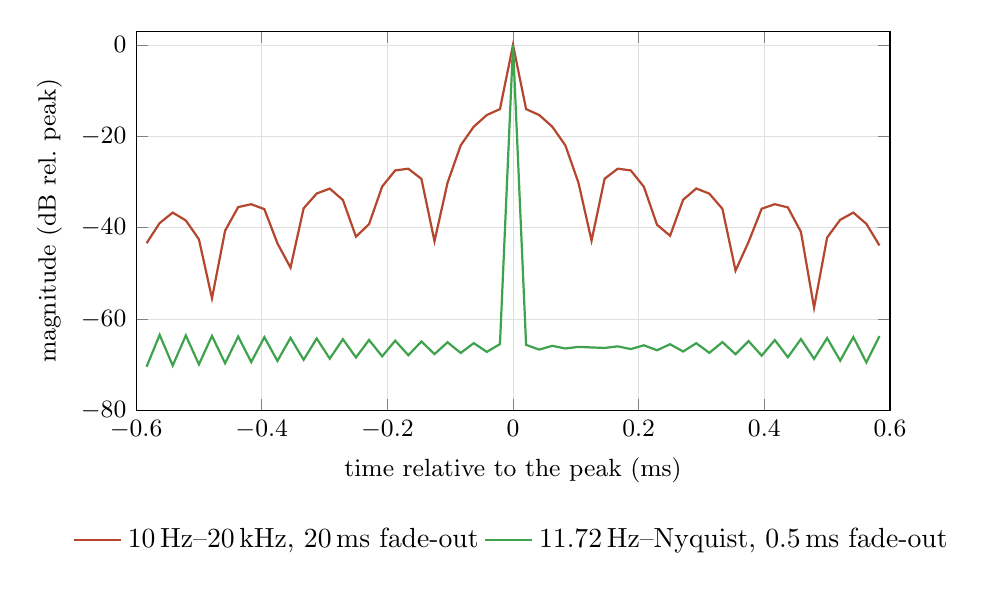
\begin{tikzpicture}
\begin{axis}[
  width=0.92\textwidth, height=6.4cm,
  xlabel={time relative to the peak (ms)},
  ylabel={magnitude (dB rel.\ peak)},
  xmin=-0.6, xmax=0.6, ymin=-80, ymax=3,
  grid=both, grid style={line width=0.2pt,draw=gray!25},
  legend style={at={(0.5,-0.28)},anchor=north,legend columns=2,draw=none},
  tick label style={font=\small}, label style={font=\small},
]
\addplot[smtred,thick,mark=none] coordinates {
(-0.5833,-43.37) (-0.5625,-38.98) (-0.5417,-36.68) (-0.5208,-38.40) (-0.5000,-42.51) (-0.4792,-55.43) (-0.4583,-40.64) (-0.4375,-35.48) (-0.4167,-34.85) (-0.3958,-35.93) (-0.3750,-43.41) (-0.3542,-48.72) (-0.3333,-35.75) (-0.3125,-32.51) (-0.2917,-31.43) (-0.2708,-33.93) (-0.2500,-41.95) (-0.2292,-39.21) (-0.2083,-30.99) (-0.1875,-27.45) (-0.1667,-27.08) (-0.1458,-29.31) (-0.1250,-42.94) (-0.1042,-30.14) (-0.0833,-21.97) (-0.0625,-17.89) (-0.0417,-15.34) (-0.0208,-14.04) (0.0000,0.00) (0.0208,-14.04) (0.0417,-15.34) (0.0625,-17.89) (0.0833,-21.98) (0.1042,-30.16) (0.1250,-42.82) (0.1458,-29.28) (0.1667,-27.07) (0.1875,-27.46) (0.2083,-31.03) (0.2292,-39.34) (0.2500,-41.75) (0.2708,-33.87) (0.2917,-31.41) (0.3125,-32.54) (0.3333,-35.85) (0.3542,-49.37) (0.3750,-43.08) (0.3958,-35.84) (0.4167,-34.84) (0.4375,-35.55) (0.4583,-40.91) (0.4792,-57.48) (0.5000,-42.14) (0.5208,-38.26) (0.5417,-36.68) (0.5625,-39.15) (0.5833,-43.87)
};
\addlegendentry{\SI{10}{\hertz}--\SI{20}{\kilo\hertz}, \SI{20}{\milli\second} fade-out}
\addplot[smtgreen,thick,mark=none] coordinates {
(-0.5833,-70.41) (-0.5625,-63.43) (-0.5417,-70.15) (-0.5208,-63.55) (-0.5000,-69.89) (-0.4792,-63.67) (-0.4583,-69.64) (-0.4375,-63.80) (-0.4167,-69.38) (-0.3958,-63.94) (-0.3750,-69.13) (-0.3542,-64.08) (-0.3333,-68.88) (-0.3125,-64.22) (-0.2917,-68.63) (-0.2708,-64.38) (-0.2500,-68.38) (-0.2292,-64.53) (-0.2083,-68.13) (-0.1875,-64.70) (-0.1667,-67.88) (-0.1458,-64.87) (-0.1250,-67.64) (-0.1042,-65.05) (-0.0833,-67.39) (-0.0625,-65.24) (-0.0417,-67.15) (-0.0208,-65.44) (0.0000,0.00) (0.0208,-65.62) (0.0417,-66.65) (0.0625,-65.83) (0.0833,-66.41) (0.1042,-66.06) (0.1250,-66.18) (0.1458,-66.29) (0.1667,-65.94) (0.1875,-66.54) (0.2083,-65.71) (0.2292,-66.80) (0.2500,-65.48) (0.2708,-67.07) (0.2917,-65.25) (0.3125,-67.36) (0.3333,-65.02) (0.3542,-67.66) (0.3750,-64.80) (0.3958,-67.98) (0.4167,-64.57) (0.4375,-68.32) (0.4583,-64.35) (0.4792,-68.68) (0.5000,-64.13) (0.5208,-69.06) (0.5417,-63.91) (0.5625,-69.47) (0.5833,-63.69)
};
\addlegendentry{\SI{11.72}{\hertz}--Nyquist, \SI{0.5}{\milli\second} fade-out}
\end{axis}
\end{tikzpicture}
\caption{Deconvolved impulse response of a pure delay, \SI{48}{\kilo\hertz},
\SI{10}{\second} sweep. The old configuration shows the slowly decaying
symmetric sinc of a band edge four kilohertz below Nyquist. The new one falls
to the floor within one sample.}
\label{fig:ir}
\end{figure}

The symmetry of the red trace is the diagnostic. A fade-out artefact would
appear on one side.

\subsection{The fade-out is nearly irrelevant, until it is not}

Removing the \SI{20}{\milli\second} fade-out from the \emph{old} band changes the
result by less than \SI{0.5}{\dB}, consistent with the \num{0.022} octave
estimate of Section~\ref{sec:mechanisms}. Cutting at the last zero crossing on
top of that changes nothing further.

Once the sweep runs to Nyquist the situation inverts, because the fade-out
becomes the only thing shaping the top edge. Figure~\ref{fig:fade} scans its
length at three sample rates.

\begin{figure}[h]
\centering
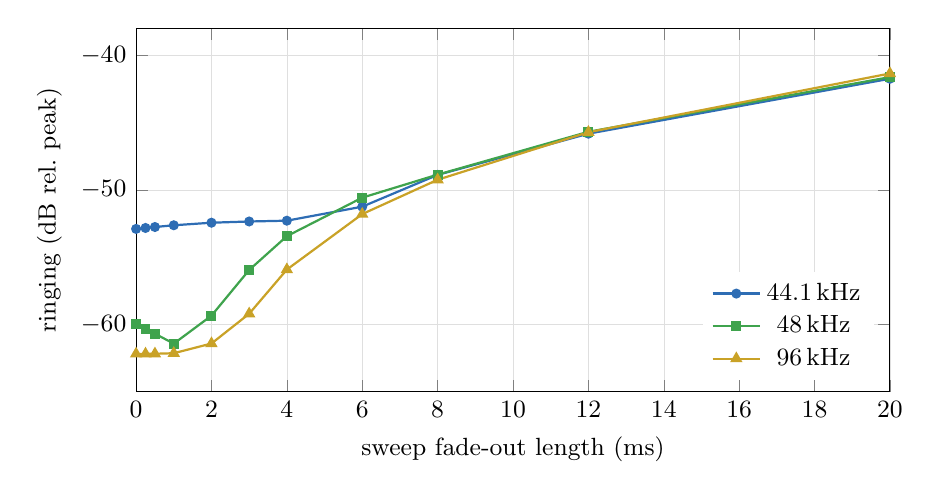
\begin{tikzpicture}
\begin{axis}[
  width=0.92\textwidth, height=6.2cm,
  xlabel={sweep fade-out length (ms)},
  ylabel={ringing (dB rel.\ peak)},
  xmin=0, xmax=20, ymin=-65, ymax=-38,
  grid=both, grid style={line width=0.2pt,draw=gray!25},
  legend style={at={(0.98,0.03)},anchor=south east,draw=none,font=\small},
  tick label style={font=\small}, label style={font=\small},
]
\addplot[smtblue,thick,mark=*,mark size=1.4] coordinates {
(0,-52.90) (0.25,-52.83) (0.5,-52.76) (1,-52.63) (2,-52.44) (3,-52.35) (4,-52.29) (6,-51.25) (8,-48.89) (12,-45.83) (20,-41.75) };
\addlegendentry{\SI{44.1}{\kilo\hertz}}
\addplot[smtgreen,thick,mark=square*,mark size=1.4] coordinates {
(0,-59.98) (0.25,-60.32) (0.5,-60.68) (1,-61.42) (2,-59.34) (3,-55.95) (4,-53.44) (6,-50.58) (8,-48.87) (12,-45.69) (20,-41.63) };
\addlegendentry{\SI{48}{\kilo\hertz}}
\addplot[smtgold,thick,mark=triangle*,mark size=1.8] coordinates {
(0,-62.18) (0.25,-62.18) (0.5,-62.17) (1,-62.13) (2,-61.41) (3,-59.20) (4,-55.92) (6,-51.80) (8,-49.25) (12,-45.72) (20,-41.36) };
\addlegendentry{\SI{96}{\kilo\hertz}}
\end{axis}
\end{tikzpicture}
\caption{Ringing against sweep fade-out length, \SI{10}{\second} sweep to
Nyquist over a whole number of octaves. Everything up to about
\SI{1}{\milli\second} sits within \SI{1}{\dB} of the optimum; beyond
\SI{4}{\milli\second} the cost is real, and the previous
\SI{20}{\milli\second} costs \SI{15}{} to \SI{25}{\dB}.}
\label{fig:fade}
\end{figure}

The curves are flat to the left and steep to the right, which is a comfortable
place to choose a value: anything short is equally good, and the penalty is
entirely on the side of being too long.

\subsection{Why the sweep cannot be cut at a zero crossing}
\label{sec:nyquist-end}

Farina's second remedy and his first are incompatible, and this appears not to
be stated anywhere in the sources.

The synchronization condition \eqref{eq:novak} already places the end of the
sweep at a zero crossing in continuous time whenever the frequency ratio is an
integer. From \eqref{eq:sweep}, the total phase is
%
\begin{equation}
  \Phi(T) \;=\; 2\pi f_1 L \Bigl( \frac{f_2}{f_1} - 1 \Bigr)
            \;=\; 2\pi k \Bigl( \frac{f_2}{f_1} - 1 \Bigr),
  \label{eq:endphase}
\end{equation}
%
so if $f_2/f_1 = 2^P$ then $\Phi(T)/2\pi = k(2^P - 1) \in \mathbb{Z}$ and
$x(T) = 0$ exactly. This is Vetter and di Rosario's phase-controlled chirp
\cite{Vetter2011}, obtained here for free from a condition the software already
imposed for a different reason.

That does not help in discrete time. The last emitted sample sits at index
$n-1$ with $n = \operatorname{round}(T f_s)$, a fraction
$\delta = T f_s - (n-1)$ of a sample before the true end. At the end of the
sweep the instantaneous frequency \emph{is} Nyquist, so the phase advances by
$2\pi f_2/f_s = \pi$ radians per sample, and the residual amplitude is
%
\begin{equation}
  \bigl| x[n-1] \bigr| \;=\; \bigl| \sin (\pi \delta) \bigr|.
  \label{eq:residual}
\end{equation}
%
Table~\ref{tab:residual} checks \eqref{eq:residual} against the generated
signal.

\begin{table}[h]
\centering
\caption{Residual amplitude of the last emitted sample, predicted by
\eqref{eq:residual} and measured on the generated sweep.}
\label{tab:residual}
\begin{tabular}{llrrr}
\toprule
$f_s$ & $T$ & $\delta$ & $|\sin(\pi\delta)|$ & measured \\
\midrule
\SI{48}{\kilo\hertz}   & \SI{10}{\second} & 0.5905 & 0.9598 & 0.9598 \\
\SI{48}{\kilo\hertz}   & \SI{5}{\second}  & 0.5149 & 0.9989 & 0.9989 \\
\SI{44.1}{\kilo\hertz} & \SI{10}{\second} & 1.1511 & 0.4572 & 0.4572 \\
\SI{96}{\kilo\hertz}   & \SI{10}{\second} & 0.9661 & 0.1062 & 0.1062 \\
\bottomrule
\end{tabular}
\end{table}

The consequence is structural, not numerical. Near Nyquist the sampled sweep is
$x[n] \approx (-1)^n \sin(\varphi_0)$: consecutive samples differ only in sign
and all of them share the magnitude $|\sin(\varphi_0)|$. There is no sample
closer to a zero crossing than any other, so searching backwards for one is
meaningless. Truncation was verified to leave both the last sample at
\num{0.960} and the ringing at \SI{-61.0}{\dB}, that is entirely unchanged.

\begin{remark}{The step is a hardware problem, not a measurement problem}
At \SI{48}{\kilo\hertz} and \SI{10}{\second} the stimulus ends by stepping from
\num{0.96} to silence. Figure~\ref{fig:fade} shows the deconvolution tolerates
this: zero fade-out is within a decibel of the best result. The reconstruction
filter of the converter, however, turns that step into a wideband transient
delivered to a tweeter at measurement level. This is the one place in the note
where the chosen value is not the one the measurement alone would pick.
\end{remark}

%==============================================================================
\section{What was implemented}
\label{sec:impl}

\subsection{The sweep band}

\code{MeasurementEngine::sweepBandFor} derives the band from the sample rate
rather than fixing it. It sets $f_2 = f_s/2$ and $f_1 = f_2 / 2^P$, choosing
$P$ to place $f_1$ as near as possible to \SI{10.5}{\hertz}:
%
\begin{equation}
  P \;=\; \operatorname{round}\bigl( \log_2 (f_2 / \SI{10.5}{\hertz}) \bigr),
\end{equation}
%
clamped to $[4, 16]$. The resulting bands are in Table~\ref{tab:bands}.

\begin{table}[h]
\centering
\caption{Sweep band produced by \code{sweepBandFor}.}
\label{tab:bands}
\begin{tabular}{lrrr}
\toprule
$f_s$ & $P$ & $f_1$ (Hz) & $f_2$ (Hz) \\
\midrule
\SI{44100}{}  & 11 & 10.767 & 22050 \\
\SI{48000}{}  & 11 & 11.719 & 24000 \\
\SI{88200}{}  & 12 & 10.767 & 44100 \\
\SI{96000}{}  & 12 & 11.719 & 48000 \\
\SI{192000}{} & 13 & 11.719 & 96000 \\
\bottomrule
\end{tabular}
\end{table}

Two constraints are satisfied at once. An integer $P$ makes $f_2/f_1$ a power of
two, so \eqref{eq:endphase} holds and the sweep ends in sine phase. And $f_1$
stays near \SI{11}{\hertz} at every rate, comfortably below the half-octave
skirt that \code{AnalysisEngine::bandWeight} places under the analysis band's
\SI{20}{\hertz} default, which reaches down to \SI{14.1}{\hertz}. Nothing
downstream loses range against the previous fixed \SI{10}{\hertz} start.

The white-noise stimulus was decoupled from this and pinned to its own fixed
\SI{10}{\hertz} to \SI{20}{\kilo\hertz} band, since it is analysed by Welch and
gains nothing from the change.

\subsection{The fade}

The fade-in is unchanged at \SI{20}{\milli\second} for both stimuli. Vetter and
di Rosario's finding that a fade-in does not raise coefficients around the
central pulse is consistent with everything measured here, and the fade-in
tapers only the bottom \num{0.02} octave in any case.

The fade-out is now split. Noise keeps \SI{20}{\milli\second}. A sweep gets
\SI{0.5}{\milli\second}, chosen from Figure~\ref{fig:fade} as the shortest value
that removes the step of \eqref{eq:residual} while remaining on the flat part of
every curve. Its cost against the best available value is at most
\SI{0.6}{\dB}, at \SI{48}{\kilo\hertz} and \SI{5}{\second}; at
\SI{96}{\kilo\hertz} it is not measurable.

\subsection{Backward compatibility}

\code{measurement.xml} already recorded $f_1$, $f_2$ and $L$ per run, and the
analysis already read them back to configure
\code{SynchronizedSweep::prepareExact}. The band therefore travels with the
measurement. Folders recorded before this change carry the old
\SI{10}{\hertz} to \SI{20}{\kilo\hertz} band in their own manifest and continue
to deconvolve exactly as they did. No migration is required and no analysis code
changed.

%==============================================================================
\section{What was deliberately not done}
\label{sec:notdone}

\subsection{The Kirkeby packing filter}

Farina's third remedy addresses the low-frequency pre-ringing that analogue
equipment contributes, by computing an inverse filter
$C(f) = \overline{H(f)} / \bigl( |H(f)|^2 + \varepsilon(f) \bigr)$ from a
reference measurement and convolving it with subsequent ones \cite{Farina2007,
Kirkeby1998}.

Simulating an AC-coupled chain, a second-order high-pass at \SI{15}{\hertz},
and building the packing filter from that same loopback, the far pre-ringing
improved from \SI{-22}{\dB} to \SI{-32}{\dB}, but the region within
\SI{1}{\milli\second} of the peak did not improve at all, and a larger
$\varepsilon$ made the result worse. On the unmodified path the AC coupling was
not even distinguishable from the band edge: \SI{-17.8}{\dB} against
\SI{-17.9}{\dB} without it.

The feature would require a reference-measurement workflow, a place to store the
reference and a rule for when it applies. For a second-order effect, dominated
by a mechanism the band change removes anyway, that is not a good trade. It is
worth revisiting only if a specific measurement chain turns out to contribute
visible low-frequency pre-ringing of its own.

\subsection{Kirkeby regularisation in the correction design}

\code{AnalysisEngine::recomputeCorrection} inverts the smoothed average as
$\overline{h}/|h|^2$ and then bends the resulting gain towards a ceiling with a
$\tanh$ soft knee. Kirkeby's additive $\varepsilon$ is the textbook alternative,
and \cite{Kirkeby1998} shows it shortens the filter's time response by pushing
poles away from the unit circle, which is exactly the property one would want
against pre-echo in a linear-phase correction.

Measured on a synthetic response with a \SI{-28}{\dB} notch, rendered through
the existing band weighting and Tukey taper, and with $\varepsilon$ chosen to
match the peak boost of the existing limiter, the two produced pre-echo within
\SI{0.1}{\dB} of each other. Fading the phase correction in the notch, which the
$\tanh$ limiter does not do and the $\varepsilon$ form does implicitly, was
worth about \SI{4}{\dB}, which is real but small and comes with its own
questions about what the corrected phase then means.

The conclusion is that the existing soft knee, combined with the complex
fractional-octave smoothing applied before inversion, already performs the
function Kirkeby's $\varepsilon$ would perform. There is no gain to collect here.

\subsection{The image-deblurring literature}

\cite{Mosleh2014} detects ringing by building Gabor filters at the blur kernel's
non-invertible frequencies and then suppresses the deblurred image's response to
them. The machinery is two-dimensional and specific to spatial images, and does
not transfer. The transferable idea is diagnostic rather than corrective:
identify the frequencies at which inversion is ill-conditioned and treat them
explicitly. In this software that would amount to flagging the bins where the
measured magnitude is so low that the correction's phase is meaningless. That
would be a user-facing diagnostic, not a change to the measurement, and it is
not pursued here.

%==============================================================================
\section{Open checks and limitations}

Two hardware questions are not settled by simulation and remain open.

\begin{enumerate}[leftmargin=*]
\item \textbf{Tweeter loading.} The stimulus now carries content up to Nyquist.
The energy per octave is unchanged, the top octave lasts about
\SI{90}{\milli\second} of a \SI{10}{\second} sweep, and the converter's
reconstruction filter attenuates the extreme top. The risk is low but it is not
zero, and it warrants one listening check at reduced level before the change is
trusted on an expensive driver.

\item \textbf{Harmonic curves.} The harmonic impulse responses extracted by
\code{estimateSweepTf} are unaffected in their separation, since
$L$ barely moves. But the range of fundamentals whose second harmonic aliases
now extends over the whole sweep, where before it began at $f_s/4$ within a band
stopping at \SI{20}{\kilo\hertz}. This is not a regression, since those
fundamentals already aliased, but the affected span of the $H_2$ to $H_5$ curves
is wider and should be read with that in mind.
\end{enumerate}

Finally, the figures in this note describe an idealised chain. In a real
measurement the floor will be set by room noise, by the loudspeaker's own
distortion and by time variance, long before it is set by the
\SI{-61}{\dB} of Table~\ref{tab:band}. The value of the change is that the
method's own contribution is now far enough below those floors to be ignored,
which was not true at \SI{-17.9}{\dB}.

%==============================================================================
\begin{thebibliography}{99}

\bibitem{Farina2000}
A.~Farina,
``Simultaneous measurement of impulse response and distortion with a swept-sine
technique'',
108th AES Convention, Paris, paper 5093, 2000.

\bibitem{Farina2007}
A.~Farina,
``Advancements in impulse response measurements by sine sweeps'',
122nd AES Convention, Vienna, 2007.

\bibitem{Kirkeby1998}
O.~Kirkeby, P.~Rubak and A.~Farina,
``Analysis of ill-conditioning of multi-channel deconvolution problems'' /
``Fast deconvolution using frequency-dependent regularization'',
Aalborg University and University of Parma, 1998.

\bibitem{Mosleh2014}
A.~Mosleh, J.~M.~P.~Langlois and P.~Green,
``Image deconvolution ringing artifact detection and removal via PSF frequency
analysis'',
in \emph{Computer Vision -- ECCV 2014}, Lecture Notes in Computer Science
vol.~8692, Springer, 2014.

\bibitem{Novak2015}
A.~Novak, P.~Lotton and L.~Simon,
``Synchronized swept-sine: theory, application, and implementation'',
\emph{J. Audio Eng. Soc.} \textbf{63}(10), 786--798, 2015.

\bibitem{Vetter2011}
K.~Vetter and S.~di Rosario,
``ExpoChirpToolbox: a Pure Data implementation of ESS impulse response
measurement'',
Rotterdam/London, 2011.

\end{thebibliography}

\end{document}
